\documentclass{article}
\usepackage{graphicx} % Required for inserting images
\usepackage{titlesec}
\usepackage{tabularx}
\usepackage[none]{hyphenat}
\setcounter{secnumdepth}{4}

\titleformat{\paragraph}
{\normalfont\normalsize\bfseries}{\theparagraph}{1em}{}
\titlespacing*{\paragraph}
{0pt}{3.25ex plus 1ex minus .2ex}{1.5ex plus .2ex}


\title{\textbf{REQUIREMENT ANALYSIS AND SPECIFICATION DOCUMENT}\\\textit{CODE KATA BATTLE}}
\author{Armando Fiorini, Samuele Motta, Vajihe Gholami}
\date{}
\begin{document}
\maketitle
\section*{INFO}
\textbf{Deliverable}: RASD\\
\textbf{Title}: Requirement Analysis and Verification Document\\
\textbf{Authors:} Armando Fiorini, Samuele Motta, Vajihe Gholami\\
\textbf{Version:} 0.0.0\\
\textbf{Date}: 18/10/2023\\
\textbf{Download page}: https://github.com/ArmaFio/FioriniMottaGholami\\
\newpage
\tableofcontents
\newpage


\section{Introduction}
\subsection{Purpose}
The purpose of this document is to outline the functionalities and requirements of CodeKataBattle (CKB), a novel platform designed to facilitate the enhancement of students' software development skills through collaborative training on code katas. Educators leverage this platform to challenge and mentor students by creating code kata battles, where teams of students engage in friendly competitions to showcase and enhance their programming skills.


\subsection{Scope}
Nowadays the world of computer science is more than ever important and present in everyone's life. For this reason, it's crucial for the teaching system to have the best
possible means to lead the students to the best possible comprehension and governance of this subject. \\
CodeKataBattle is a platform supposed to allow Educators to create coding tournaments in which students can compete, in teams or on their own, to improve their skills in any type of programming language.\\\\
In order to ensure that the system allows Educators to manage all the settings and rules of the tournaments (number of battles, allowed Students' team size, score assignment rules, proper programming language \dots), to which students can subscribe.\\
All the Students logged into the app receive a notification each time a tournament has been created.\\
Students involved in a tournament can create teams (according to the tournament's rules), and then it's time for them to start coding: through Git they will be allowed to receive the problem's text and to submit their solution, within a configured time range.\\
The solutions will then be evaluated, by the system or the Educator, and will contribute to defining the final rank of the tournament.\\\\
Their stats in tournaments will be public and visible in the account of a student, as well as their achieved badges: a badge is a reward that is created by an Educator, who defines the requirement(s) to gain it: the badges can be assigned to one or more students and are relative to a single tournament, at the end of which they are eventually assigned.

\subsection{Definitions, Acronyms, Abbreviations} 
\subsubsection{Definitions}
\textbf{Educator:} user who signs up to use the system as a mean to improve the programming skills of his students, he can create Tournaments
and badges.\\\\
\textbf{\\Student:} user who signs up to improve their skills, participating to tournaments which are created by the educators. \\\\\\
\textbf{\\Tournament:} coding challenge, consisting in a certain number of battles.\\\\\\
\textbf{\\Team:} group of students, formed to join a tournament and work together to win the battles.\\\\\\
\textbf{\\Battle:} every single challenge the tournament is composed of. \\\\\\
\textbf{\\(Gamification) Badge:} achievement that is created from an educator, and can be obtained from Students satisfacting the estabilished requirements.\\\\
\textbf{}
\subsubsection{Acronyms}
\begin{itemize}
    \item \textbf{CKB}: CodeKataBattle
    \item \textbf{RASD}: Requirement Analysis and Specification Document
    \item \textbf{UI}: User Interface
    \item \textbf{UML}: Unified Modelling Language
\end{itemize}

\subsubsection{Abbreviations}
\begin{itemize}
    \item \textbf{$[Gn]$}: the n-th goal of the system.
    \item \textbf{$[Wn]$}: the n-th world phenomena.
    \item \textbf{$[SWn]$}: the n-th shared phenomena controlled by the world.
    \item \textbf{$[SMn]$}: the n-th shared phenomena controlled by the machine.
    \item \textbf{$[Dn]$}: the n-th domain assumption.
    \item \textbf{$[FRn]$}: the n-th functional requirement.
\end{itemize}

\subsection{Overview}
\subsubsection{Goals}
These are the goals that the system is supposed to achieve:\\\\
$[G1]$ Educators and students can subscribe to the application creating their personal account \\
$[G2]$ Educators create Tournaments in which students can compete \\
$[G3]$ Students subscribe to the tournaments \\
$[G4]$ Students compete, in teams or on their own, in many battles, the results of which will determine the final rank of the tournament  \\
$[G5]$ Students can reach achievements that permit them to gain badges for their account \\
$[G6]$ Educators create badges and define requirements to achieve them \\
\newpage
      \subsubsection{Phenomena}
        {\setlength{\leftskip}{2em}
            \paragraph{World Phenomena}
            $[W1]$ User downloads the application\\
            $[W2]$ An Educator decides in class to use the application to organize a coding tournament\\
            $[W3]$ A Student decides to join a battle\\
            $[W4]$ A Student contacts some mates to form a team\\
            $[W5]$ A Student pushes a solution on GitHub\\

            \paragraph{Shared Phenomena}
            \textbf{Controlled by the world and observed by the machine} \\\\
            $[SW1]$ A user creates an account and logs into the application\\
            $[SW2]$ An Educator creates a tournament\\
            $[SW3]$ A Student, or a team of students, joins a tournament\\
            $[SW4]$ An Educator creates a badge\\
            $[SW5]$ An Educator creates a battle\\
            $[SW6]$ A User decides to visualize his or another one's account page\\
            $[SW7]$ An Educator performs manual evaluation of the submitted solutions for a battle
\\\\
            \textbf{Controlled by the machine and observed by the world}\\\\
            $[SM1]$ Student receives a notification: a tournament has been created \\
            $[SM2]$ A Student is notified that the time for submitting their solution is terminating\\
            $[SM3]$ A Student is shown he has achieved a badge\\
            $[SM4]$ A User is shown his account or another one's, with all the badges and stats\\
            $[SM5]$ The system evaluates a solution submitted by a student and gives them the score
            }

\newpage

\section{Overall Description}
\subsection{Product Perspective}
\subsubsection{Scenarios}
\begin{enumerate}
  \item \textbf{An Educator creates a tournament\\}John wants to create a coding tournament to make his students train their
  coding skills: he signs in into the system and he clicks on the "My Tournaments" button on his home page, then he clicks on "Create new Tournament":
  at this point he can set the name of the tournament the list of collaborators (Colleagues that can create battles in the context of that tournament) and a subscription
  deadline for the students who want to join the tournament, after that time the subscription will be closed and the tournament will result as started.\\
  When he clicks on confirm the tournament has finally been created: now all the students will be notified and can join it.\\
  \item \textbf{An Educator creates a battle\\}An Educator wants to create a new battle for the tournament: once he has signed in he can go in to "My Tournaments" section
  and select a started tournament.\\
  If the tournament has no ongoing battles the function "Create new battle" is enabled: the Educator can then manage the battle settings.
  In particular he has to configure:
  \begin{itemize}
    \item The programming language(s) students are allowed to use for coding that the evaluating system will recognize
    \item The maximum number of students for each team that will compete in the battle
    \item The registration deadline for the battle
    \item The submission deadline for the solutions
    \item The evaluation system options (Totally automated, manual checking)
  \end{itemize}
  He has finally to submit the text of the problem for the battle: it will be automatically uploaded in a repository created by the system at the registration
  deadline and the students will be automatically given the link to see it and start coding.\\
  \newpage
  \item \textbf{An Educator creates a Badge\\}An Educator wants to create a gamification badge: badges exist in the context of a tournament, so the Educator clicks on an ongoing tournament
  in "My Tournaments" section and then on "Create a Badge".\\
  Once reached this section the Educator is shown the list of parameters offered by the system which represent properties regarding which conditions can be built, including values of commits number, code length, code speed, joined battles
  and so on; he also writes a brief description of the requirement in the dedicated section.
  Once the conditions are written the Educator uploads an image for the badge and gives it a name, and eventually clicks on "confirm": now the badge is available for all students of that tournament.\\
  \item \textbf{A Students joins a tournament\\} Mark has been notified that a new tournament has been created and wants to join it: he can click on the notification, that will redirect him directly on the tournament page, or search for it by himself clicking on "Join a Tournament" in "My Tournaments"
  section of his homepage. 
  Once he has found the tournament he clicks join and he's in: he can now see the list of the incoming battles to join them on his own or with his team.\\
  \item \textbf{A Students joins a battle\\} Mark has seen that a battle is starting in a tournament he has joined and has decided to join it with 2 friends, that have also subscribed to the tournament.\\
  He selects the tournament from him ones list and then selects the battle: he can then see his team for the battle, to which he can invite people who has subscribed to the tournament pushing the '+' button, and a confirmation button.\\
  He invites his 2 friends selecting them from a list containing the subscribers and after some time he receives a notification that the invites have been accepted: in that moment he comes back to the battle page and sees his friend's name 
  appeared in his team: now he clicks on confirm and the registration is confirmed, they have to wait for the beginning of the battle.
  \newpage 
  \item \textbf{A Student achieves a badge\\} Paul is competing in a tournament, last battle of which has just ended: since the Educator who has created the tournament defined a badge for the team 
  having committing the biggest number of times, the system verifies that condition and Paul is resulting as the gainer of the badge.\\
  The system then sends a notification to him: when he sees it he goes to his profile homepage and in "My Badges" section he sees the new badge he has achieved.\\
  Eventually, clicking on it, he can see the information about the badge, including the description of the requirement from which he is now able to know
  how he has gain the achievement.


\end{enumerate}

\subsubsection{Domain Class Diagram}
\subsubsection{Statecharts}
\subsection{Product Functions}
\subsubsection{Sign Up and Login}
These function will be available to all the users: during the sign up procedure every one has to insert an e-mail and a password: these will be also the credentials to log in into the account that is being created.\\
The inserted e-mail will be verified from the system with a confirmation e-mail sent to the user.\\
Once this step is done the user will have to insert their personal data: Name, Surname, an username that will be the one who will be seen by the other users, and the type of user (Educator or Student).
\subsubsection{Tournament creation}
Each Educator can use the system to create tournaments for single students or for teams: in the single player tournaments, if the Educator enables the option, the students can form teams for a single battle, the score of which will be added to the single score of each component.\\
When creating a tournament an Educator has to set the list of available programming languages, the number of battles and to give it a name, they can in addition choose to set it as private protecting it with an alphanumerical access key.\\
The tournaments can also been handled by more than one Educator: collaborators can be added from creation pages.
In case of teams tournaments the educator will be asked to choose the maximum number of Students per team.
Once an Educator has created a tournament every user in the system is notified and can join it.
The creator has to set a subscription deadline: as the deadline expires the tournament status passes from opened to ongoing and no one can join it anymore.
\subsubsection{Tournament subscription}
Each student can subscribe to a tournament: once they have found a tournament in which they want to compete, exploring the list or searching it in there by name or creator, they can click and join it, inserting the access key if it's required. 
In case of teams tournaments Students will have to build their teams since the beginning: they can so invite whoever they want to subscribe to the tournament and join their team; when the team is ready the team leader can confirm the registration and the game is done.
\subsubsection{Battle creation}
In the context of an ongoing tournament Educators have to set the options of each battle before making it start: if the tournament is for single players and team battles are enabled the Educator has to choose the maximum team size in that battle, the language(s) for that specific battle picked from the tournament's ones, and to set the subscription and solution submission deadline.
He has also to decide if the solutions will be evaluated totally by the system or if he also wants to manually check the solutions at the end of the battle.
After having done that the Educator has to upload on the app the text and test cases for the problem that the Students have to solve in that battle: when the battle begins a public repository containing the text will be created on GitHub and made available to all Students involved in the battle
Once all this has been done the Educator confirms the creation of the battle: all the Students that are subscribed to the tournament are notified and the timer for the registration starts.
\subsubsection{Battle joining}
Each student subscribed to a tournament can join its battles: they receive a notification every time a new battle is ready to start and they have time to join it until the deadline set by the Educator has expired.\\
If the tournament is for single players, the educator can allow students to create teams in the context of each single battle: the team components will be assigned the same score but in the tournament ranking they will still be considered as separate challengers; the team will be dissolved as the battle ends.\\
As the deadline for subscribing expires each competing student will be allowed to see the link of the repository where they will find the text of the exercise with test cases and will upload their solution.
\newpage
\subsubsection{Code Evaluation}
The System, during a battle, will use static code analysis tools (such as Pylint) to give a score to each competitor: the score is assigned each time a solution is pushed on the gitHub repository so that a live provisional rank is always visible for all the duration of the battle to all the Students involved. 
When the battle ends, and after the eventual manual evaluation by the Educator, Students will be able to see the final scores of all the competitors in the rank of the battle, and also the updated tournament rank.\\
The score is a number from 0 to 100, determined basing on criteria like correctness but also time and space efficiency and so on.
\subsubsection{Gamification Badges}
Educators are allowed, in the context of a tournament, to create Gamification Badges.\\
Badges are achievements that the Students can gain satisfying a requirement.\\
When creating a badge, an educator has to give it a name, optionally an image, and to write a brief description of the requirement : these are the things that students will be able to see.\\
To make the system be able to analyze the requirement and eventually assign the badge when it's necessary, the Educator has also to write it as a boolean condition built on parameters given by the System.\\
Even if a parameter value changes during the battle the system verifies the conditions that have been created and, if someone has satisfied it, gives him the badge and sends him a notification.\\
\subsubsection{Stats and Rankings}
Each user is allowed to explore other accounts: in particular the tournament ranks (ended and ongoing ones) and the badges of a user are public; every one can see them clicking on their account.

\subsection{User Characteristics}
The system is designed to interact with the following two different kinds of users:
\subsubsection{Educator}
An educator is an user who registered through the CKB app by creating an "educator account", it is able to create tournaments and battles, inviting collaborators in the tournament, evaluate the solutions provided by the students and create badges for each tournament (optional).
\subsubsection{Student}
A student is an user who registered through the CKB app by creating a "student account", it is able to join tournaments and battles, invite other students in their current team and submit solutions for the battles in which it joined.
\subsection{Assumptions, dependencies and constraints}

\subsubsection{Domain Assumptions}
The following are the domain assumptions that need to be satisfied for the correct behaviour of CKB. Since those situations are out of the control of the system, they are taken as granted.\\\\
$[D1]$ User must have an internet connection.\\
$[D2]$ User must have a GitHub account.\\
$[D3]$ User must know how to use GitHub in the proper way (push, pull, branch, etc.).\\
$[D4]$ Connection between systems must be reliable.\\
$[D5]$ Test cases provided by educators must be correct.\\
$[D6]$ GitHub works as expected.\\

\section{Specific Requirements}
\subsection{External Interface Requirements}
\subsubsection{User Interfaces}
In this section is presented the user interface through which both students and educators can:
\begin{itemize}
    \item Log in
    \item Sign Up
    \item Access personal dashboard
\end{itemize}
The needs of educators and students are not the same, therefore they are going to get access to different views:\\
Educators have access to specific views that allow them to handle tournaments and battles while students must be able to join tournaments and battles, as well as invite members in their group.



\begin{figure}
    \hspace*{-2cm}
    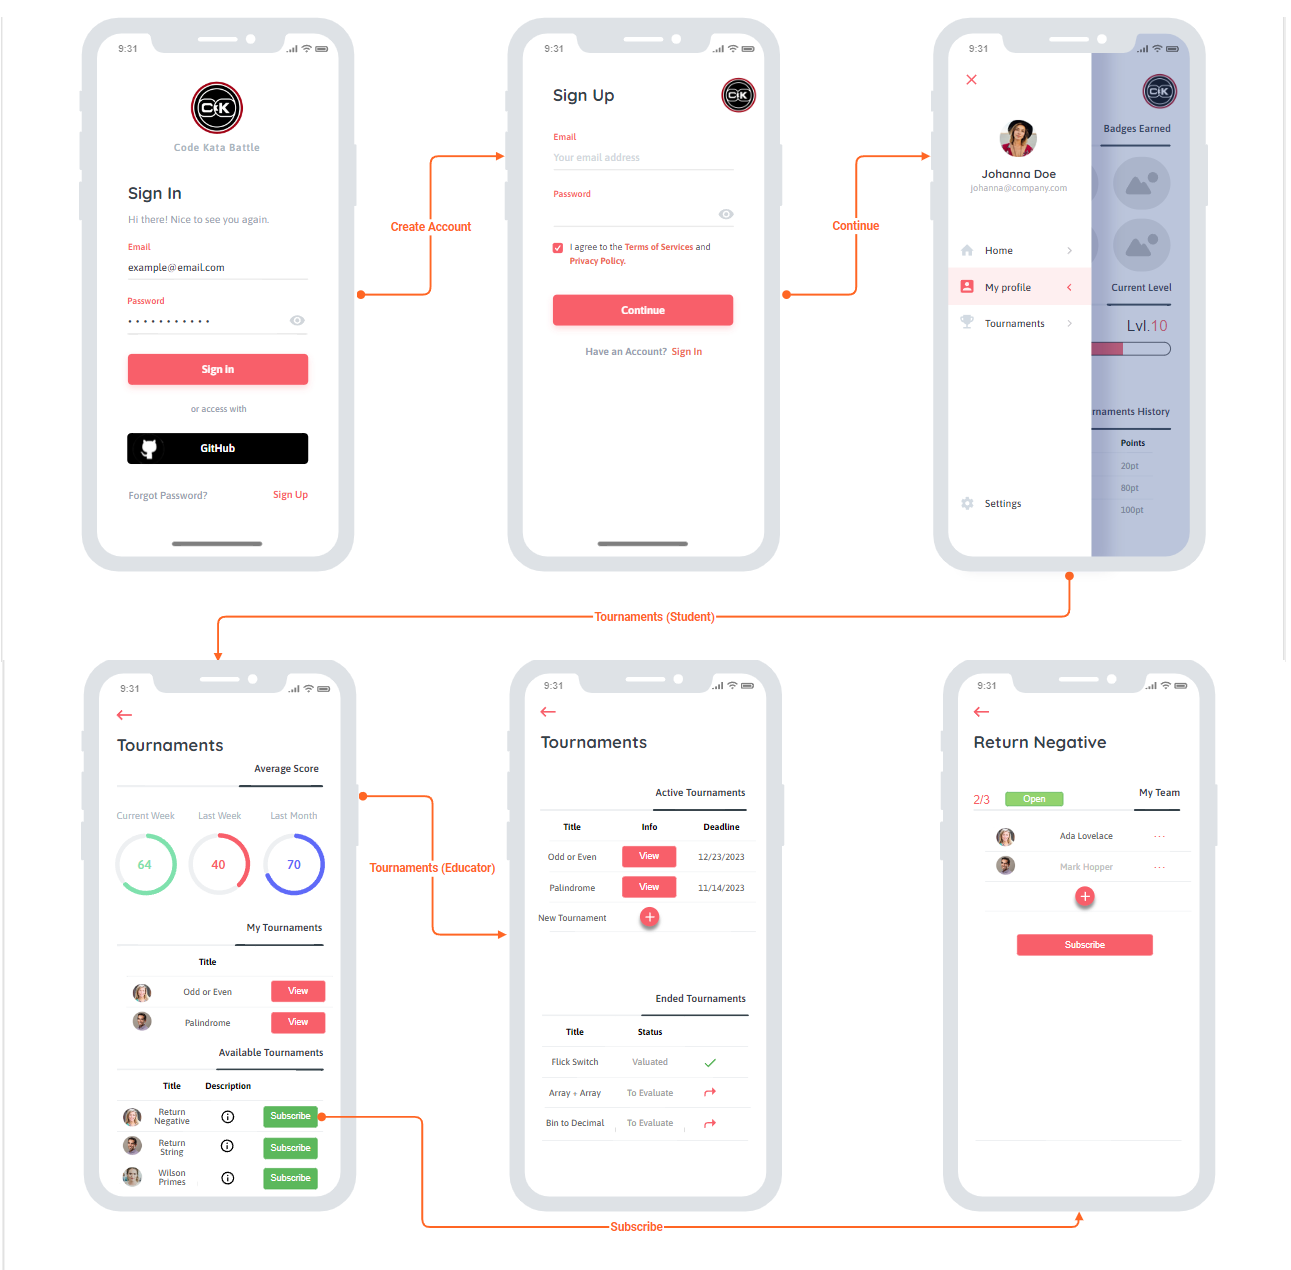
\includegraphics[scale=1.5]{UI.png}
    \caption{User Interface}
\end{figure}
\newpage
\subsubsection{Hardware Interfaces}

The system offers to the users different services (see paragraph \textbf{2.2}) that can be accessed by any device with an internet connection whether it's through app or web app.
                            
\subsubsection{Software Interfaces}



\subsection{Functional Requirements}
$[FR1]$ The system allows Users (Students and Educators) to sign up.\\
$[FR2]$ The system allows Users (Students and Educators) to login.\\
$[FR3]$ The system allows Educators to create tournaments.\\
$[FR4]$ The system allows Educators to set the maximum number of students per team in a tournament.\\
$[FR5]$ The system allows Educators to set the number of battles in a tournament.\\
$[FR6]$ The system allows Educators to create battles.\\
$[FR7]$ The system allows Educators to choose whether and when the scores will be assigned in a totally automatic way or also through a manual verification by themselves\\
$[FR8]$ The system allows Educators to create badges for a specific tournament.\\
$[FR9]$ The system allows Educators to state the requirements for achieving a badge.\\
$[FR10]$ The system allows Users to join a tournament.\\
$[FR11]$ The system allows Users to see the ranking in tournaments and achieved badges of every signed up student in the system.\\
$[FR12]$ The system allows Educators to see the list of the active tournaments they have created.\\
$[FR13]$ The system allows Users to see the list of the active tournaments they have joined.\\

\newpage

\section{Alloy}
\includegraphics[scale = 0.7]{Untitled-1.pdf}

\section{Effort Spent}
\begin{center}
\textbf{Armando Fiorini} \\
\vspace{10px}
    \begin{tabularx}{0.8\textwidth} { 
  | >{\centering\arraybackslash}X 
  | >{\centering\arraybackslash}X | }
 \hline
 \textbf{Chapter} & \textbf{Hours Spent} \\
 \hline
 1 & TBD  \\
 \hline
 2 & TBD \\
 \hline
 3 & TBD \\
 \hline
 4 & TBD \\
 \hline
\end{tabularx}

\vspace{10px}
\textbf{Samuele Motta} \\
\vspace{10px}
\begin{tabularx}{0.8\textwidth} { 
  | >{\centering\arraybackslash}X 
  | >{\centering\arraybackslash}X | }
 \hline
 \textbf{Chapter} & \textbf{Hours Spent} \\
 \hline
 1 & TBD  \\
 \hline
 2 & TBD \\
 \hline
 3 & TBD \\
 \hline
 4 & TBD \\
 \hline
\end{tabularx}

\vspace{10px}
\textbf{Vajihe Gholami} \\
\vspace{10px}
\begin{tabularx}{0.8\textwidth} { 
  | >{\centering\arraybackslash}X 
  | >{\centering\arraybackslash}X | }
 \hline
 \textbf{Chapter} & \textbf{Hours Spent} \\
 \hline
 1 & TBD  \\
 \hline
 2 & TBD \\
 \hline
 3 & TBD \\
 \hline
 4 & TBD \\
 \hline
\end{tabularx}

\end{center}

\section{References}
\end{document}